\documentclass[11pt,a4paper]{article}

% -------------------------------------------------
% Packages
% -------------------------------------------------
\usepackage[utf8]{inputenc}
\usepackage[T1]{fontenc}
\usepackage[english]{babel}
\usepackage{siunitx}
\usepackage{graphicx}
\usepackage{amsmath}
\usepackage{booktabs}
\usepackage{geometry}
\usepackage{fancyhdr}
\usepackage{hyperref}
\usepackage{eurosym}
\geometry{margin=2.5cm}
\setlength{\parskip}{1em}
\setlength{\parindent}{0em}

\pagestyle{fancy}
\fancyhf{}
\rhead{Framework for GNNs on TUDataset}
\lhead{Erik Deinzer}
\rfoot{\thepage}

% -------------------------------------------------
% Title Information
% -------------------------------------------------
\title{Framework for GNNs on TUDataset}
\author{Erik Deinzer and Felix Glatzel}
\date{\today}

% -------------------------------------------------
% Document
% -------------------------------------------------
\begin{document}
	
	% Title Page
	\maketitle
	\thispagestyle{empty}
	\vfill
	\begin{center}
		\large
		Project Report for \\[0.5cm]
		\textbf{Prof. Rizzi} \\[0.5cm]
		\textbf{Prof. De Santis} \\[0.5cm]
		Sapienza University of Rome \\[0.5cm]
		\today
	\end{center}
	\vfill
	\newpage
	
	% Table of Contents
	\tableofcontents
	\newpage
	
	\section{Introduction}
	Graph-structured data is increasingly prevalent across a wide range of domains, including chemistry, biology, social networks, and recommendation systems. Traditional machine learning techniques often struggle to handle such data due to its non-Euclidean nature. Graph Neural Networks (GNNs) have emerged as a powerful class of models designed to learn representations from graph data by leveraging the underlying structure of nodes and edges.
	
	This project explores the application of GNNs to graph classification tasks using real-world datasets from the TUDataset collection. Specifically, we design and implement a modular and extensible pipeline capable of loading, preprocessing, training, and evaluating models on multiple datasets, including MUTAG, PROTEINS, and ENZYMES. These datasets are commonly used benchmarks in the GNN research community and represent various challenges in terms of graph size, sparsity, heterogeneity, and domain-specific semantics.
	
	Our objectives are threefold: (1) to deepen our understanding of how GNNs can be applied to graph classification problems; (2) to gain practical experience with PyTorch Geometric (PyG) and the TUDataset API; and (3) to analyze and compare the performance of different GNN architectures across datasets with diverse structural characteristics.
	
	In addition to implementing a working framework, we provide a detailed analysis of the structure and nature of each dataset, including an examination of what the nodes and edges represent, whether the graphs are small or large, sparse or dense, and whether they are homogeneous or heterogeneous. We also survey relevant literature to identify key papers that have used these datasets and report their benchmark results for comparison.
	
	This report presents our methodology, findings, and conclusions. It is structured as follows: Section 2 provides background on GNNs and related work; Section 3 introduces the datasets; Section 4 outlines the pipeline implementation; Section 5 presents the experiments and results; and Section 6 concludes the report and suggests possible improvements.
	
	\section{Methods}
	
	\subsection{Datasets}
	In the context of graph classification, several properties are used to describe and compare graph datasets. These characteristics help determine how challenging a dataset is and what modeling strategies may be appropriate.
	
	\paragraph{Small vs. Large Graphs} 
	This refers to the number of nodes and edges per individual graph in the dataset. 
	\begin{itemize}
		\item \textbf{Small graphs} usually have tens of nodes and edges (e.g., MUTAG), making them computationally light and less structurally complex.
		\item \textbf{Large graphs} can have hundreds or thousands of nodes and edges, requiring more memory and processing power (e.g., datasets like REDDIT-BINARY or COLLAB).
	\end{itemize}
	
	\paragraph{Sparse vs. Dense Graphs} 
	This characterizes the ratio of the actual number of edges to the maximum possible number of edges.
	\begin{itemize}
		\item A graph is \textbf{sparse} if it has relatively few edges compared to the number of nodes (common in molecular or protein datasets).
		\item A graph is \textbf{dense} if it has many edges and a high degree of node connectivity.
	\end{itemize}
	Formally, sparsity can be approximated by the edge density:
	$\text{Density} = \frac{2 \cdot |E|}{|V| \cdot (|V| - 1)}$
	where $|E|$ is the number of edges and $|V|$ is the number of nodes. With Density $D \geq 0.4$, a graph is denoted as dense in the following, a graph with $D \leq 0.1$ as very sparse and a graph with $D \approx 1$ as fully connected..
	
	\paragraph{Homogeneous vs. Heterogeneous Graphs}
	\begin{itemize}
		\item \textbf{Homogeneous graphs} contain only one type of node and one type of edge. Most classical GNN benchmarks (like MUTAG) fall in this category.
		\item \textbf{Heterogeneous graphs} include multiple types of nodes and/or edges, each potentially carrying different semantic information. For example, in biological datasets, nodes may represent different molecule components or protein substructures with diverse attributes.
	\end{itemize}
	
	\paragraph{Attributed vs. Non-Attributed Graphs}
	\begin{itemize}
		\item In \textbf{attributed graphs}, nodes (and sometimes edges) carry feature vectors or labels, which can be used as input to GNN models.
		\item \textbf{Non-attributed graphs} only provide connectivity information, and node/edge features must be inferred or embedded manually.
	\end{itemize}
	
	\paragraph{Labeled vs. Unlabeled Graphs}
	\begin{itemize}
		\item \textbf{Labeled graphs} provide a target class (e.g., "mutagenic" or "non-mutagenic") for each graph, necessary for supervised learning.
		\item \textbf{Unlabeled graphs} are more suitable for unsupervised or self-supervised learning approaches.
	\end{itemize}
	
	\paragraph{Multi-class vs. Binary Classification}
	This refers to the number of target classes:
	\begin{itemize}
		\item \textbf{Binary classification} tasks (e.g., MUTAG, PROTEINS) distinguish between two labels.
		\item \textbf{Multi-class classification} tasks (e.g., ENZYMES) require assigning one label from more than two categories.
	\end{itemize}
	
	
	
To evaluate the performance of Graph Neural Networks (GNNs) in graph classification tasks, we employ three well-established datasets from the TUDataset collection: \textbf{MUTAG}, \textbf{PROTEINS}, and \textbf{ENZYMES}. These datasets are drawn from domains such as chemistry and bioinformatics and are widely used in benchmarking GNN architectures due to their distinct structural properties and classification challenges. In the following sections, we present a detailed description of each dataset, including the semantics of nodes and edges, the size and density of the graphs, and the nature of their labels.

\subsection*{MUTAG}

The MUTAG dataset consists of 188 chemical compounds, each modeled as an undirected graph. The classification task is to predict whether each compound exhibits mutagenic activity on a specific bacterium strain (\textit{Salmonella typhimurium}). This is a binary classification problem.

\paragraph{Graph Structure:}
Each graph represents a molecule where:
\begin{itemize}
	\item \textbf{Nodes} correspond to atoms in the molecule, such as Carbon (C), Oxygen (O), Nitrogen (N), etc. Each node is associated with a discrete label that identifies the atom type.
	\item \textbf{Edges} represent chemical bonds between atoms. These are undirected and unweighted, with no bond-type information explicitly provided in the basic version of the dataset.
\end{itemize}

\paragraph{Characteristics:}
\begin{itemize}
	\item \textbf{Number of graphs:} 188
	\item \textbf{Average number of nodes per graph:} 17.93
	\item \textbf{Average number of edges per graph:} 19.79
		\item \textbf{Mean Density:} $D \approx 0.096$
	\item \textbf{Classes:} 2 (mutagenic, non-mutagenic)
	\item \textbf{Type:} Small, very sparse, homogeneous, labeled, attributed
\end{itemize}

\paragraph{Scientific Usage:}
MUTAG has been used extensively as a benchmark in kernel-based and neural network-based graph learning models. Notable references include:
\begin{itemize}
	\item Weisfeiler-Lehman subtree kernel \cite{shervashidze2011weisfeiler}
	\item Graph Convolutional Networks (GCN) \cite{kipf2017semi}
	\item Graph Isomorphism Network (GIN) \cite{xu2019powerful}
\end{itemize}

\subsection*{PROTEINS}

The PROTEINS dataset is derived from the protein data bank and contains 1,113 protein graphs. The classification task is to determine whether each protein is an enzyme or a non-enzyme, resulting in a binary classification problem.

\paragraph{Graph Structure:}
Each graph models the secondary structure of a protein:
\begin{itemize}
	\item \textbf{Nodes} correspond to secondary structure elements (SSEs), such as alpha helices or beta sheets. Nodes are labeled with discrete types and may carry additional structural features.
	\item \textbf{Edges} connect SSEs that are in close spatial proximity or connected sequentially. These edges are undirected and encode structural relationships.
\end{itemize}

\paragraph{Characteristics:}
\begin{itemize}
	\item \textbf{Number of graphs:} 1,113
	\item \textbf{Average number of nodes per graph:} 39.06
	\item \textbf{Average number of edges per graph:} 72.82
		\item \textbf{Mean Density:} $D \approx 0.098$
	\item \textbf{Classes:} 2 (enzyme, non-enzyme)
	\item \textbf{Type:} Medium-sized, very sparse, heterogeneous, labeled, attributed
\end{itemize}

\paragraph{Scientific Usage:}
PROTEINS is a common benchmark in both classical and deep graph learning literature. It was used in:
\begin{itemize}
	\item Deep Graph Kernels \cite{yanardag2015deep}
	\item Message Passing Neural Networks (MPNNs) \cite{morris2020tudataset}
	\item Geometric deep learning benchmarks \cite{dwivedi2020benchmarking}
\end{itemize}

\subsection*{ENZYMES}

ENZYMES contains 600 protein graphs that are classified into one of six enzyme classes as defined by the Enzyme Commission (EC) number classification. This is a multi-class classification problem.

\paragraph{Graph Structure:}
Each graph represents a protein, modeled similarly to the PROTEINS dataset:
\begin{itemize}
	\item \textbf{Nodes} denote SSEs in the protein structure, labeled by type and possibly enriched with additional feature information.
	\item \textbf{Edges} indicate spatial or sequential proximity between SSEs. These are undirected and generally sparse.
\end{itemize}

\paragraph{Characteristics:}
\begin{itemize}
	\item \textbf{Number of graphs:} 600
	\item \textbf{Classes:} 6 (corresponding to EC enzyme classes)
	\item \textbf{Average number of nodes per graph:} 32.63
	\item \textbf{Average number of edges per graph:} 62.14
	\item \textbf{Mean Density:} $D \approx 0.12$
	\item \textbf{Type:} Medium-sized, sparse, heterogeneous, labeled, attributed
\end{itemize}

\paragraph{Scientific Usage:}
ENZYMES presents a more complex classification challenge due to its multi-class nature and greater intra-class variability. It has appeared in:
\begin{itemize}
	\item GIN benchmark experiments \cite{xu2019powerful}
	\item TUDataset benchmarking \cite{morris2020tudataset}
	\item Comparative studies between graph kernels and deep models \cite{yanardag2015deep}
\end{itemize}
	
	\subsection{Summary Table}
	
	\begin{table}[h]
		\centering
		\begin{tabular}{lcccccc}
			\toprule
			\textbf{Dataset} & \textbf{\# Graphs} & \textbf{Avg. Nodes} & \textbf{Avg. Edges} & \textbf{Classes} & \textbf{Graph Type}\footnotemark & \textbf{Domain} \\
			\midrule
			MUTAG    & 188  & 17.93 & 19.79 & 2 & S, SP, HO & Chemistry \\
			PROTEINS & 1113 & 39.06 & 72.82 & 2 & M, SP, HE & Biology \\
			ENZYMES  & 600  & 32.63 & 62.14 & 6 & M, SP, HE & Biology \\
			\bottomrule
		\end{tabular}
		\caption{Overview of the main properties of the selected TUDatasets. 
		}
	\footnotetext*{\footnotesize(S=Small, SP=Sparse, HO=Homogenous, M=Medium, HE=Heterogenous)}
	\end{table}

	\subsection{Graph Neural Network Architectures}
	
	Graph Neural Networks (GNNs) are designed to process graph-structured data by leveraging the relationships (edges) between entities (nodes). The key idea is to iteratively update node representations by aggregating information from their neighbors. In this section, we discuss four prominent GNN architectures: Graph Convolutional Networks (GCN), Graph Isomorphism Networks (GIN), Graph Attention Networks (GAT), and GraphSAGE. Each of these models defines a different message passing and aggregation strategy.
	
	\subsection{Graph Convolutional Network (GCN)}
	
	Graph Convolutional Networks (GCNs) were introduced in \cite{kipf2017semi} as an extension of the convolution operation to graph-structured data. GCNs perform a form of \emph{neighborhood averaging}, where each node updates its representation based on the features of its neighbors and itself.
	
	The forward propagation rule for a single GCN layer is:
	
	\begin{equation}
		\mathbf{H}^{(l+1)} = \sigma\left( \mathbf{\tilde{D}}^{-1/2} \mathbf{\tilde{A}} \mathbf{\tilde{D}}^{-1/2} \mathbf{H}^{(l)} \mathbf{W}^{(l)} \right)
	\end{equation}
	
	\begin{figure}[h]
		\centering
		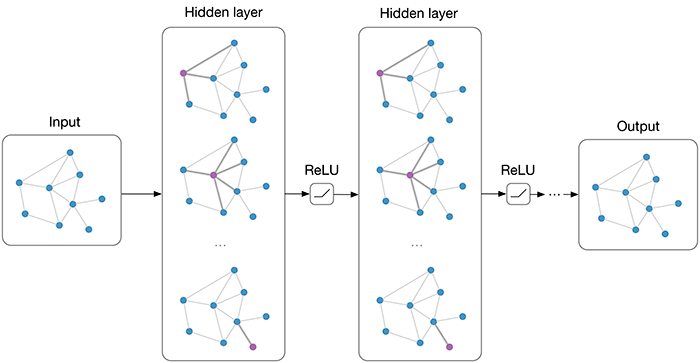
\includegraphics[width=0.7\textwidth]{gcn.png}
		\caption{Graph Convolutional Neural Network \cite{pic:gcn}.}
	\end{figure}

	\paragraph{Explanation of Symbols:}
	\begin{itemize}
		\item $\mathbf{H}^{(l)}$ is the matrix of node features at layer $l$; each row is the feature vector for one node.
		\item $\mathbf{H}^{(0)}$ is the input feature matrix (e.g., atom types).
		\item $\mathbf{\tilde{A}} = \mathbf{A} + \mathbf{I}$ is the adjacency matrix of the graph with added self-loops.
		\item $\mathbf{\tilde{D}}$ is the diagonal degree matrix of $\tilde{A}$, where $\tilde{D}_{ii} = \sum_j \tilde{A}_{ij}$.
		\item $\mathbf{W}^{(l)}$ is a trainable weight matrix at layer $l$.
		\item $\sigma$ is a non-linear activation function (typically ReLU).
	\end{itemize}
	
	The normalization $\mathbf{\tilde{D}}^{-1/2} \mathbf{\tilde{A}} \mathbf{\tilde{D}}^{-1/2}$ ensures that feature aggregation is scaled properly, especially for nodes with high degree. GCNs are efficient and perform well on many tasks, but they are limited in expressivity due to their linear nature and tendency to oversmooth node features across layers.
	
	\subsection{Graph Isomorphism Network (GIN)}
	
	The Graph Isomorphism Network (GIN), proposed in \cite{xu2019powerful}, is a GNN architecture specifically designed to match the discriminative power of the Weisfeiler-Lehman (WL) test — a classical test for graph isomorphism.
	
	The update rule in GIN is:
	
	\begin{equation}
		\mathbf{h}_v^{(l+1)} = \text{MLP}^{(l)} \left( (1 + \epsilon) \cdot \mathbf{h}_v^{(l)} + \sum_{u \in \mathcal{N}(v)} \mathbf{h}_u^{(l)} \right)
	\end{equation}
	
	\begin{figure}[h]
		\centering
		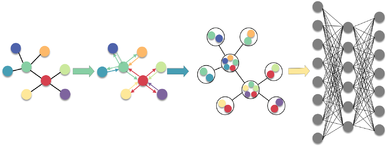
\includegraphics[width=0.7\textwidth]{gin.png}
		\caption{Node update process of a  GIN layer \cite{pic:gin}.}
	\end{figure}

	\paragraph{Explanation of Symbols:}
	\begin{itemize}
		\item $\mathbf{h}_v^{(l)}$ is the feature vector of node $v$ at layer $l$.
		\item $\mathcal{N}(v)$ denotes the set of neighboring nodes of $v$.
		\item $\epsilon$ is a learnable or fixed scalar that determines the importance of the central node's own features.
		\item $\text{MLP}^{(l)}$ is a multi-layer perceptron applied after aggregation.
	\end{itemize}
	
	Unlike GCNs, which average the features, GIN performs a \emph{sum aggregation} followed by a non-linear transformation, which retains more unique structural information. This design choice makes GIN theoretically more powerful for distinguishing non-isomorphic graphs. GIN performs particularly well in graph classification tasks such as MUTAG and ENZYMES.
	
	\subsection{Graph Attention Network (GAT)}
	
	Graph Attention Networks (GATs), introduced in \cite{velivckovic2018graph}, apply an attention mechanism to graphs. Instead of treating all neighbors equally, GAT learns to assign different importance (attention scores) to each neighbor.
	
	The update rule for GAT is:
	
	\begin{equation}
		\mathbf{h}_v^{(l+1)} = \sigma\left( \sum_{u \in \mathcal{N}(v)} \alpha_{vu}^{(l)} \cdot \mathbf{W}^{(l)} \mathbf{h}_u^{(l)} \right)
	\end{equation}
	
	\paragraph{Explanation of Symbols:}
	\begin{itemize}
		\item $\mathbf{h}_v^{(l)}$ and $\mathbf{h}_u^{(l)}$ are the feature vectors of node $v$ and its neighbor $u$.
		\item $\mathbf{W}^{(l)}$ is a trainable weight matrix.
		\item $\alpha_{vu}^{(l)}$ is the attention coefficient from node $v$ to node $u$, learned via:
		\[
		\alpha_{vu}^{(l)} = \frac{
			\exp\left(\text{LeakyReLU}\left(\mathbf{a}^T [\mathbf{W}^{(l)} \mathbf{h}_v^{(l)} \, \| \, \mathbf{W}^{(l)} \mathbf{h}_u^{(l)}]\right)\right)
		}{
			\sum_{k \in \mathcal{N}(v)} \exp\left(\text{LeakyReLU}\left(\mathbf{a}^T [\mathbf{W}^{(l)} \mathbf{h}_v^{(l)} \, \| \, \mathbf{W}^{(l)} \mathbf{h}_k^{(l)}]\right)\right)
		}
		\]
		\item $\mathbf{a}$ is a trainable attention vector; $\|$ denotes vector concatenation.
	\end{itemize}
	
	\begin{figure}[h]
		\centering
		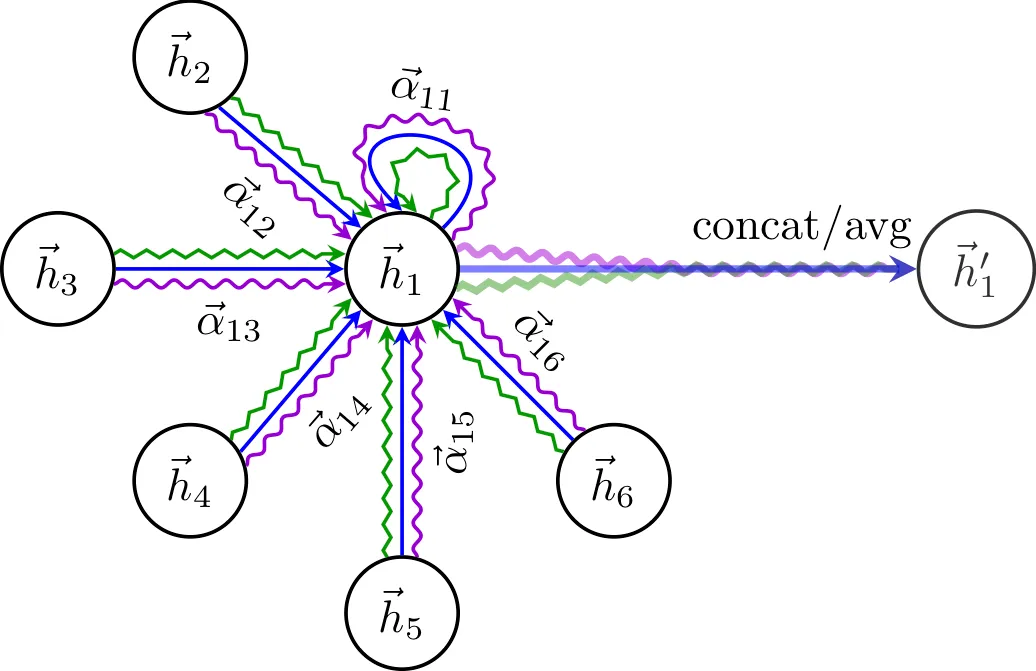
\includegraphics[width=0.7\textwidth]{gat.png}
		\caption{Graph Attention Mechanism \cite{pic:gat}.}
	\end{figure}

	By learning attention scores, GAT can focus on the most relevant parts of a node's neighborhood, which is useful for datasets where not all connections are equally informative. It is particularly effective in social network data, though its performance in small molecular graphs is also competitive.
	
	\subsection{GraphSAGE}
	
	GraphSAGE (Graph Sample and Aggregate), introduced in \cite{hamilton2017inductive}, was designed for \emph{inductive learning}, i.e., making predictions on unseen graphs. Unlike full-neighborhood aggregation, GraphSAGE samples a fixed-size neighborhood and aggregates features using various strategies (mean, max-pool, LSTM).
	
	The generic update rule is:
	
	\begin{equation}
		\mathbf{h}_v^{(l+1)} = \sigma\left( \mathbf{W}^{(l)} \cdot \text{AGG}^{(l)} \left( \left\{ \mathbf{h}_v^{(l)} \right\} \cup \left\{ \mathbf{h}_u^{(l)} \, | \, u \in \mathcal{N}(v) \right\} \right) \right)
	\end{equation}

	\begin{figure}[h]
		\centering
		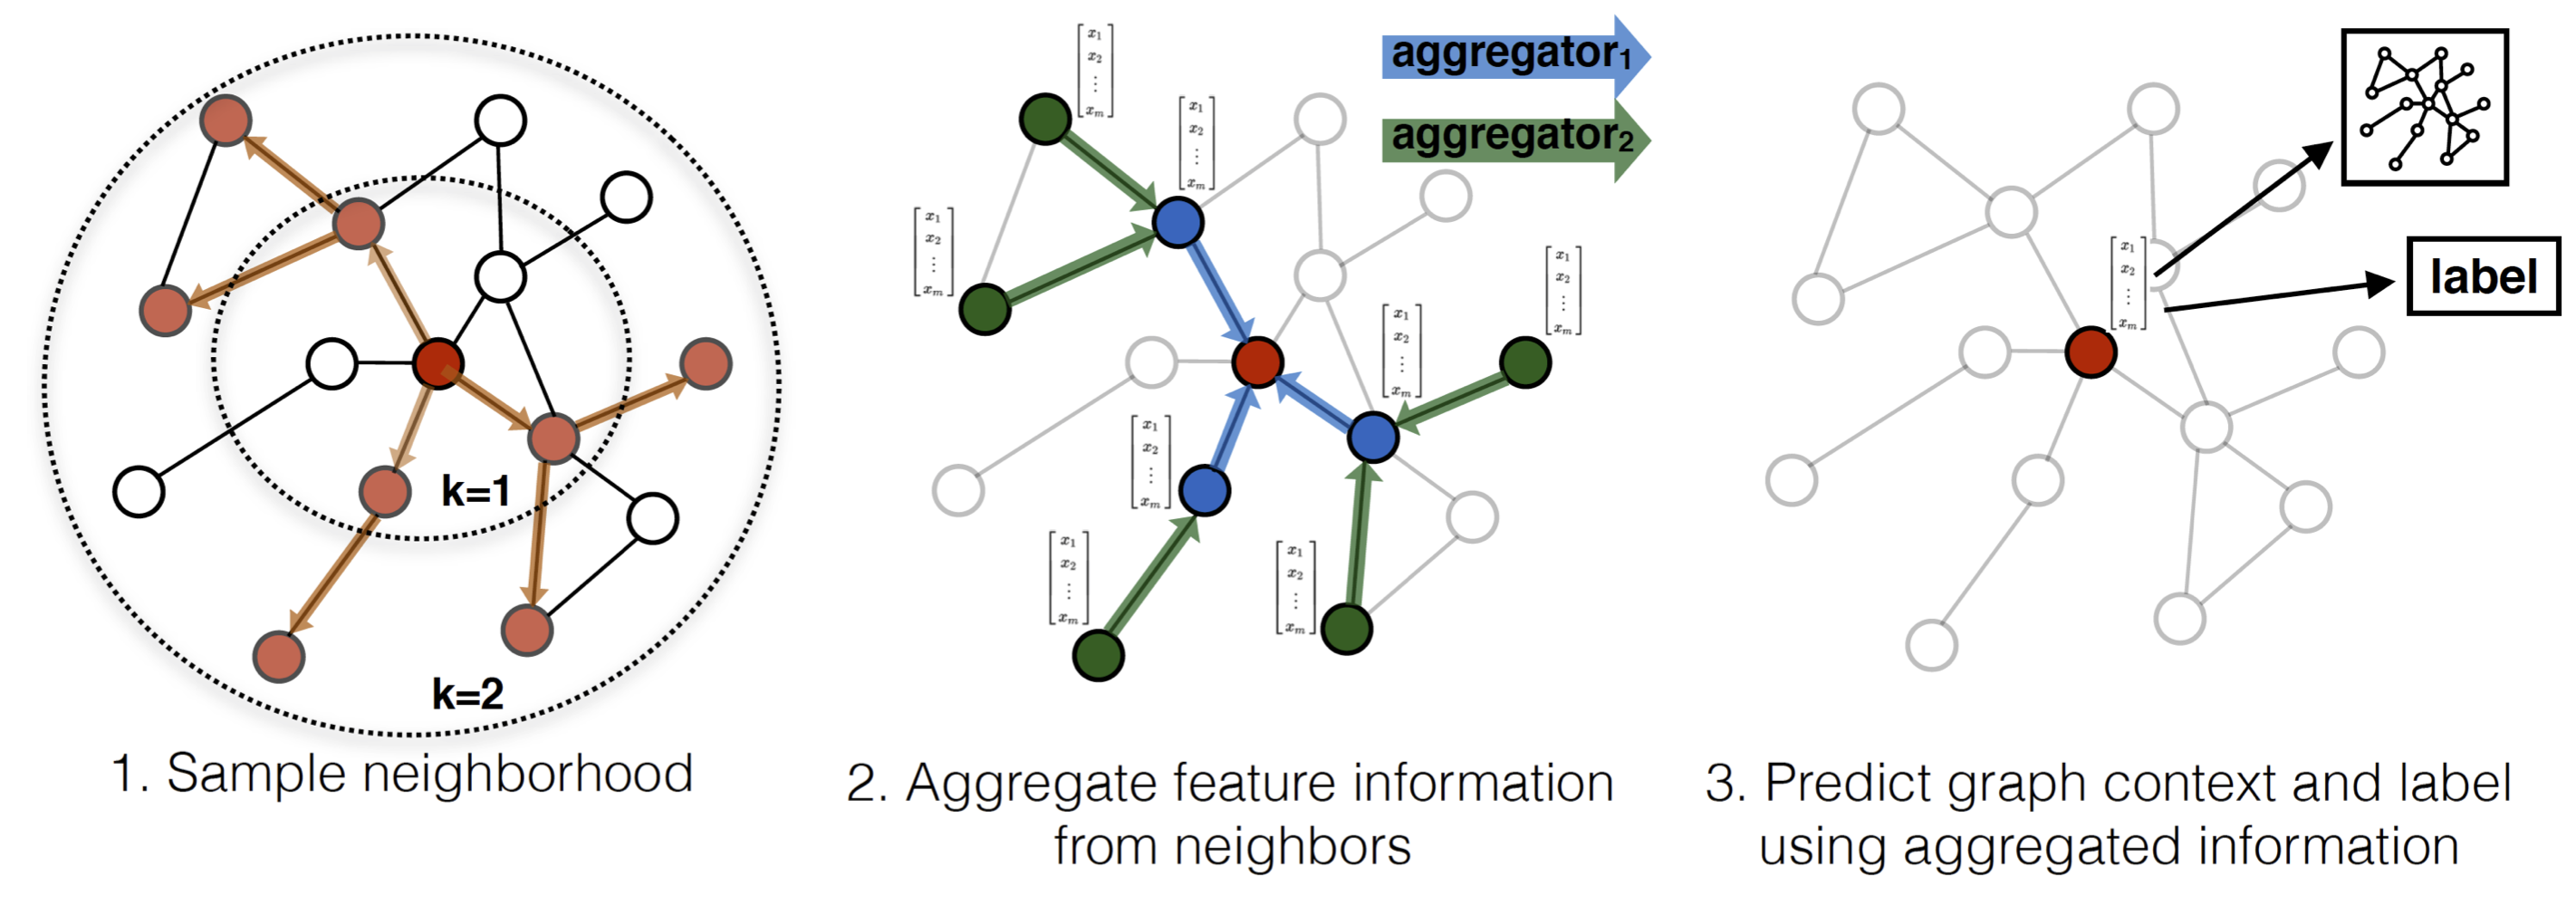
\includegraphics[width=0.7\textwidth]{graphsage.png}
		\caption{Graphsage Node update \cite{pic:graphsage}.}
	\end{figure}
	
	\paragraph{Explanation of Symbols:}
	\begin{itemize}
		\item $\text{AGG}^{(l)}$ is an aggregation function (e.g., mean, LSTM, max-pooling).
		\item $\mathbf{h}_v^{(l)}$ is the current node embedding at layer $l$.
		\item $\mathbf{W}^{(l)}$ is a trainable weight matrix.
		\item $\sigma$ is a non-linear activation function.
	\end{itemize}
	
	GraphSAGE is particularly scalable for large graphs, such as citation or social networks, due to its sampling approach. It also enables efficient inference on previously unseen nodes and graphs.
	
	
	
	
	%END DOCUMENT - APPEND REFERENCES
	\bibliographystyle{plain}
	\bibliography{references}
	
\end{document}